\documentclass{siproblemset}

\usepackage{multicol}

% SI Session Information
\course{MTH 1321}
\sessionnum{2}
\sessiondate{1/20/20}

\warmup{Concept Review}
\topic{What is a limit?}
\topic{Limit Laws}
\topic{Understanding Limits}
\topic{Solving Limits using Limit Laws}
\cooldown{Rates of Change and Continuity}

% Worksheet Information
\title{Rates of Change and\linebreak Introduction to Limits}
\sections{Sections 2.1-2.3}
\withnamespace

\begin{document}
    \maketitle
    
    \activity{Warmup}{Limit Concept Overview}{Work \textbf{alone} then share your answers with a \textbf{partner}. Try not to use your notes.}{15 minutes}
    
    \frq{In your own words, describe what a limit is and/or what it does.}
    \tinyspace
    
    \frq{What are the condition(s) for a limit (such as $\lim\limits_{x\to 2}f(x)$) to exist?}
    \tinyspace
    
    \frq{What are the basic limit laws?}
    \begin{center}
        \begin{tabular}{ |c|c|c| } 
            \hline
            \multicolumn{3}{|c|}{If $\lim\limits_{x\to c}f(x)=L$ and $\lim\limits_{x\to c}g(x)=M$ exist, then:}\\[4ex]
            \hline
            \textbf{Law Name} & \textbf{Law Definition} & \textbf{Constraints (if applicable)} \\ 
            \hline
            Constant Law & \hspace{3in} & \\ 
            &&\\
            \hline
            Identity Law & \hspace{3in} & \\ 
            &&\\
            \hline
            Sum Law & \hspace{3in} & \\ 
            &&\\
            \hline
            Difference Law & \hspace{3in} & \\ 
            &&\\
            \hline
            Constant Multiple Law & \hspace{3in} & \\ 
            &&\\
            \hline
            Product Law & \hspace{3in} & \\ 
            &&\\
            \hline
            Quotient Law & \hspace{3in} & \\ 
            &&\\
            \hline
            Power-Root Law & \hspace{3in} & \\ 
            &&\\
            \hline
        \end{tabular}
    \end{center}
    \pagebreak
    
    \activity{Activity 1}{Understanding Limits}{Work in a \textbf{group of 2 or 3 people sitting near you} to answer these questions. Try not to use your notes.}{30 minutes}
    
    \begin{multipartquestion}
        Find the value of the following limits. If the limit does not exist, find the values of the left-hand and right-hand limits.
        \begin{multicols}{2}
            \frq{$\lim\limits_{x\to -2}f(x)$ and $\lim\limits_{x\to 2}f(x)$}
            \mbox{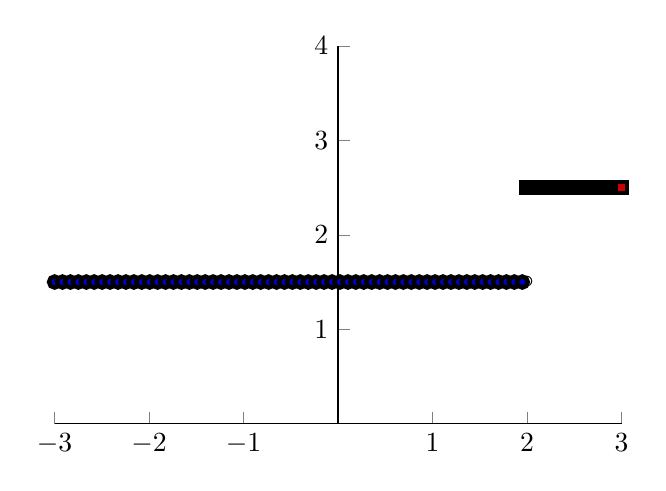
\begin{tikzpicture}[baseline=(current bounding box.north)]
                \begin{axis}[
                    x=1.2cm,
                    y=1.2cm,
                    xmin=-3,
                    xmax=3,
                    ymin=0,
                    ymax=4,
                    axis x line*=middle,
                    axis y line*=middle,
                    every axis plot/.append style={ultra thick},
                    samples=60
                    ]
                    \addplot+[black, domain=-3:1.95] {1.5};
                    \addplot+[black, domain=2:3] {2.5};
                    \node at (2,1.5) {$\circ$};
                    \node at (2,2.5) {\textbullet};
                \end{axis}
            \end{tikzpicture}}
            \Tinysp
        
            \frq{[(c)]$\lim\limits_{x\to -2}f(x)$ and $\lim\limits_{x\to 1}f(x)$}
            \mbox{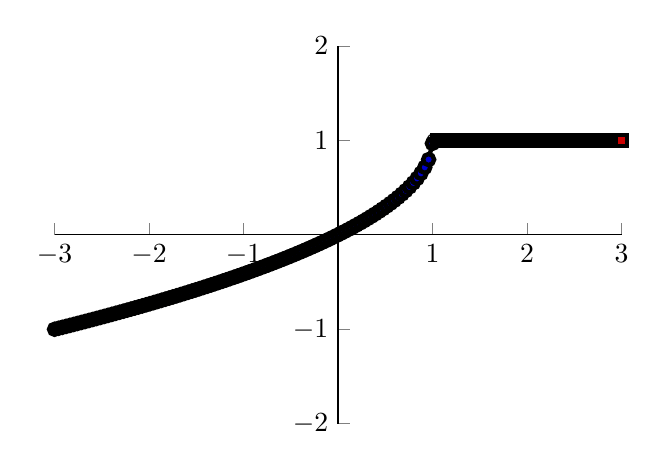
\begin{tikzpicture}[baseline=(current bounding box.north)]
                \begin{axis}[
                    x=1.2cm,
                    y=1.2cm,
                    xmin=-3,
                    xmax=3,
                    ymin=-2,
                    ymax=2,
                    axis x line*=middle,
                    axis y line*=middle,
                    every axis plot/.append style={ultra thick},
                    samples=100
                    ]
                    \addplot+[black, domain=-3:0.999] {1-sqrt(-x+1)};
                    \addplot+[black, domain=1.05:3] {1};
                    \node at (1,1) {$\circ$};
                \end{axis}
            \end{tikzpicture}}
            \Tinysp
        
            \frq{[(b)]$\lim\limits_{x\to -1}f(x)$ and $\lim\limits_{x\to 0}f(x)$}
            \mbox{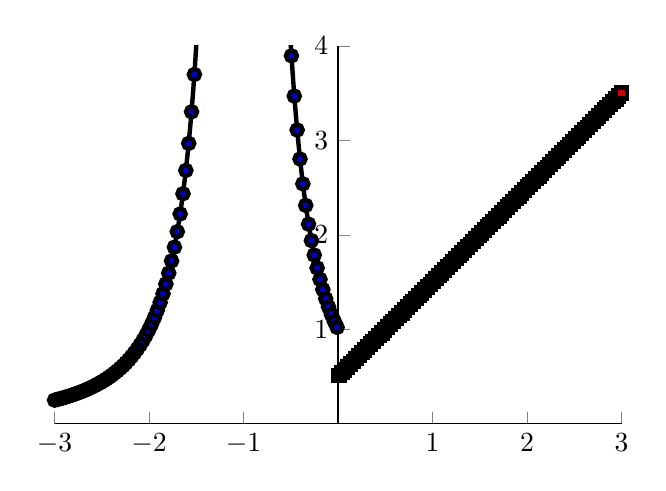
\begin{tikzpicture}[baseline=(current bounding box.north)]
                \begin{axis}[
                    x=1.2cm,
                    y=1.2cm,
                    xmin=-3,
                    xmax=3,
                    ymin=0,
                    ymax=4,
                    axis x line*=middle,
                    axis y line*=middle,
                    every axis plot/.append style={ultra thick},
                    samples=100
                    ]
                    \addplot+[black, domain=-3:-0.01,restrict y to domain =-20:100] {1/(x+1)^2};
                    \addplot+[black, domain=0.01:3] {x+1/2};
                    \node at (0,1) {$\circ$};
                    \node at (0,0.5) {\textbullet};
                \end{axis}
            \end{tikzpicture}}
            \Tinysp
        
            \frq{$\lim\limits_{x\to 0}f(x)$ and $\lim\limits_{x\to 2.5}f(x)$}
            \mbox{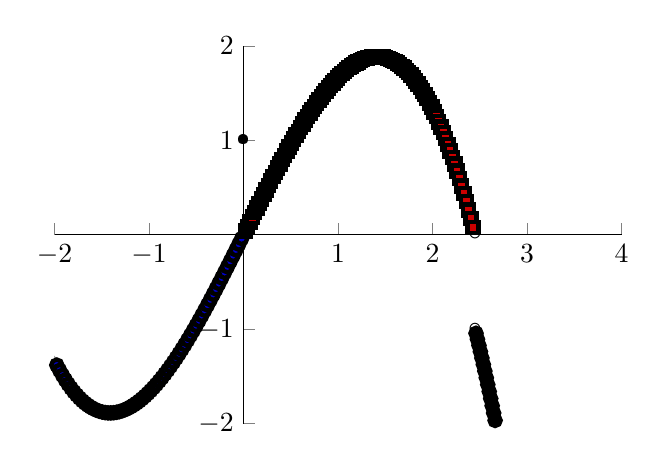
\begin{tikzpicture}[baseline=(current bounding box.north)]
                \begin{axis}[
                    x=1.2cm,
                    y=1.2cm,
                    xmin=-2,
                    xmax=4,
                    ymin=-2,
                    ymax=2,
                    axis x line*=middle,
                    axis y line*=middle,
                    every axis plot/.append style={ultra thick},
                    samples=100
                    ]
                    \addplot+[black, domain=-3:-0.02,restrict y to domain =-20:100] {-x^3/3+2*x};
                    \addplot+[black, domain=0.02:2.43,restrict y to domain =-20:100] {-x^3/3+2*x};
                    \addplot+[black, domain=2.46:4,restrict y to domain =-20:100] {-x^3/3+2*x-1};
                    \node at (0,0) {$\circ$};
                    \node at (0,1) {\textbullet};
                    \node at (2.45,0) {$\circ$};
                    \node at (2.45,-1) {$\circ$};
                \end{axis}
            \end{tikzpicture}}
            \Tinysp
        \end{multicols}
    \Tinysp
    \end{multipartquestion}
    \newpage
    \begin{multipartquestion}
        Estimate the value of the following limits. If the limit does not exist, estimate the values of the left-hand and right-hand limits.
        \frq{$\lim\limits_{x\to 0}\dfrac{x^2-4x}{x-4}$\hfill
        \begin{tabular}{ |c|c|c|c|c| } 
            \hline
            \textbf{$x$} & \textbf{$-0.001$} & \textbf{$-0.0001$} & \textbf{$0.0001$} &\textbf{ $0.001$} \\
            \hline
            \textbf{$f(x)$} & \hspace{2cm} & \hspace{2cm} & \hspace{2cm} & \hspace{2cm} \\
            \hline
        \end{tabular}}
        \Smallsp
        \frq{$\lim\limits_{x\to -3}\dfrac{1}{x+3}$\hfill
            \begin{tabular}{ |c|c|c|c|c| } 
                \hline
                \textbf{$x$} & \textbf{$-3.001$} & \textbf{$-3.0001$} & \textbf{$-2.9999$} &\textbf{ $-2.999$} \\
                \hline
                \textbf{$f(x)$} & \hspace{2cm} & \hspace{2cm} & \hspace{2cm} & \hspace{2cm} \\
                \hline
        \end{tabular}}
    \end{multipartquestion}
    \Smallsp
    
    \activity{Activity 2}{Solving Limits Using Limit Laws}{Work in a \textbf{group of 2 or 3 people with the same color worksheet as you} to answer these questions. Try not to use your notes.}{30 minutes}
    \mcq{Evaluate the following limits by using the Basic Limit Laws. \textit{Show what law you are using at each part.}}{
        \task $\lim\limits_{x\to25}\dfrac{3\sqrt{x}-\frac15x}{(x-20)^2}$
        \largesp
        \task $\lim\limits_{x\to 4}\dfrac{x^2+1}{\left(x^3+2\right)\left(x^4+1\right)}$
    }
    \Largesp
    \mcq{Evaluate the following limits by using the Basic Limit Laws. \textit{Show what law you are using at each part.}$$\lim\limits_{x\to2}g(x)=3~~~\text{and}~~~\lim\limits_{x\to2}h(x)=-2$$}{
        \task $\lim\limits_{x\to2}\dfrac{g(x)+5x}{h(x)^2}$
        \normalsp
        \task $\lim\limits_{x\to2}\frac12h(x)\sqrt{g(x)}$
        \normalsp
        \task $\lim\limits_{x\to2}\dfrac{g(x)^2}{g(x)-1}$
        \normalsp
        \task $\lim\limits_{x\to2}\dfrac{g(x)^{3/2}}{2h(x)}$
    }
    \newpage
    
    \activity{Cooldown}{Looking Back, Looking Forward}{Test your knowledge of previous topics and upcoming topics by answering these questions \textbf{alone}. Try not to use your notes.}{15 minutes}
    
    \begin{multipartquestion}
        \frq{What is the slope of the secant line to the function $f(x)$ between the points corresponding to $x=a$ and $x=a+h$?}
        \tinyspace
        \frq{This slope is also called the \underline{\hspace{2in}}.}
        \frq{What does each axis need to represent in order for the slope of the secant line to be called the ``average velocity''?}
        \tinyspace
        \frq{Taking the limit of the average rate of change as $h\to 0$ gives what quantity?}
        \tinyspace
    \end{multipartquestion}

    \frq{What is an asymptote? \textit{Both define the term and draw an example.}}
    \smallspace
\end{document}